\section{Modular Coding and Linking}

\begin{definition}{From source code to executable Program}\\
Compile/Asseble each Module:
Results in an object file for each module

Link all object files together:
Creates a single executable file

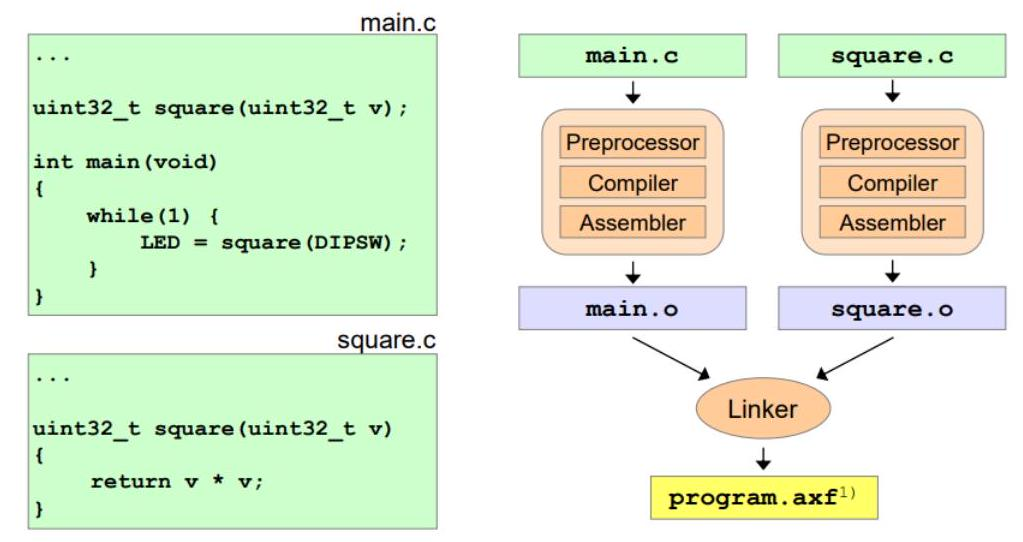
\includegraphics[width=\linewidth]{images/2024_12_29_79e6b22f503fb7b4f718g-10(2)}
\end{definition}

\begin{concept}{Tool Chain Components}
Essential tools for development:

\begin{minipage}[t]{0.5\textwidth}
  \begin{itemize}
    \item \textbf{Compiler (armcc)}:
      \begin{itemize}
        \item Translates C to assembly
        \item Performs optimizations
        \item Generates object files
      \end{itemize}
    \item \textbf{Assembler (armasm)}:
      \begin{itemize}
        \item Processes assembly code
        \item Creates object files
        \item Handles directives
      \end{itemize}
  \end{itemize}
\end{minipage}
\begin{minipage}[t]{0.5\textwidth}
  \begin{itemize}
    \item \textbf{Linker (armlink)}:
      \begin{itemize}
        \item Combines object files
        \item Resolves references
        \item Creates executable
      \end{itemize}
    \item \textbf{Library Manager (armar)}:
      \begin{itemize}
        \item Creates/maintains libraries
        \item Adds/removes object files
        \item Archives multiple objects
      \end{itemize}
  \end{itemize}
\end{minipage}
\end{concept}

\begin{theorem}{Guidelines for Modular Programming}
Key design principles:
\begin{itemize}
  \item \textbf{High Cohesion}: Group related functionality together
    \begin{itemize}
      \item Each module fulfills a single defined task
      \item Lean external interface
    \end{itemize}
  \item \textbf{Low Coupling}: Minimize dependencies between modules
    \begin{itemize}
      \item Clear and minimal interfaces
      \item Easy to modify individual modules
    \end{itemize}
  \item \textbf{Information Hiding}: Split interface from implementation
    \begin{itemize}
      \item Don't expose unnecessary details
      \item Maintain freedom to change internals
    \end{itemize}
\end{itemize}
\end{theorem}

\begin{corollary}{Benefits of Modular Programming}
Key advantages:

\textbf{Team Development}: Multiple developers working on same codebase
    \begin{itemize}
      \item Clear ownership of modules
    \end{itemize}
\textbf{Code Organization}: Logical partitioning/grouping of functionality
    \begin{itemize}
      \item Easier code reuse an better maintainability/understandability
    \end{itemize}
\textbf{Development Efficiency}:
    \begin{itemize}
      \item Individual module testing
      \item Faster compilation (only recompile changed modules)
      \item Reusable library creation
    \end{itemize}
\textbf{Language Integration}: Mix C and assembly modules
    \begin{itemize}
      \item Language-specific optimizations (best of both worlds)
    \end{itemize}
\end{corollary}

\begin{remark}
Important considerations:
\begin{itemize}
  \item Use consistent naming conventions
  \item Document module interfaces clearly
  \item Consider initialization dependencies
  \item Test modules independently
  \item Maintain version control
  \item Document build requirements
\end{itemize}
\end{remark}



\subsubsection{Module Interfaces and Linkage}

\begin{definition}{Module Linkage}

\begin{minipage}{0.44\textwidth}
  Keywords for controlling \\module interfaces:\\
  \begin{itemize}
    \item \textbf{EXPORT}: Make symbol\\ available to other modules
    \item \textbf{IMPORT}: Use symbol \\from another module
    \item Internal symbols: \\Neither IMPORT \\nor EXPORT
  \end{itemize}
\end{minipage}
\begin{minipage}{0.55\textwidth}
  \vspace{-6mm}
  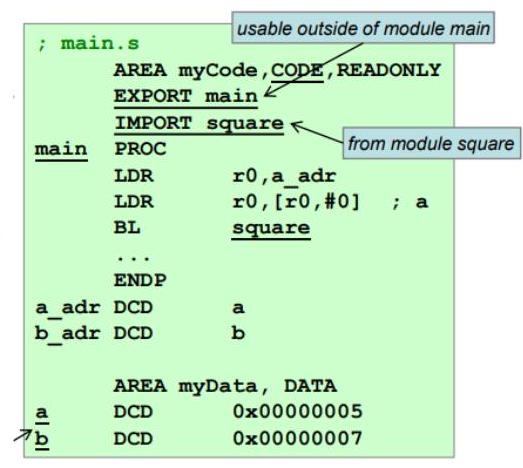
\includegraphics[width=\linewidth]{images/2024_12_29_79e6b22f503fb7b4f718g-10(1)}
\end{minipage}
\end{definition}



\begin{KR}{Working with Linkage in ARM Assembly}

\textbf{1. Exporting symbols:} Use EXPORT directive before symbol definition
\begin{itemize}
  \item Only export symbols needed by other modules
  \item Can export both code and data symbols
\end{itemize}

\textbf{2. Importing symbols:} Use IMPORT directive before symbol usage
\begin{itemize}
  \item Import must match exactly with export name
  \item Import before first use of symbol
\end{itemize}

\textbf{3. Internal symbols:} No EXPORT/IMPORT directive
\begin{itemize}
  \item Only visible within current module
  \item Used for module-private implementation
\end{itemize}
\end{KR}


\begin{example2}{Multiple Module Linkage}\\
Example of two interacting modules:

Module 1 (math\_ops.s):
\begin{lstlisting}[language=armasm, style=basesmol]
    AREA |.text|, CODE, READONLY
    EXPORT add_and_square
    IMPORT square_value    ; From module 2
    
add_and_square PROC
    PUSH    {R4, LR}
    ADDS    R4, R0, R1    ; Add parameters
    MOVS    R0, R4        ; Prepare for square
    BL      square_value  ; Call imported function
    POP     {R4, PC}
    ENDP
    END
\end{lstlisting}

Module 2 (square.s):
\begin{lstlisting}[language=armasm, style=basesmol]
    AREA |.text|, CODE, READONLY
    EXPORT square_value
    
square_value PROC
    PUSH    {LR}
    MULS    R0, R0, R0    ; Square the input
    POP     {PC}
    ENDP
    END
\end{lstlisting}
\end{example2}


\begin{remark}
Important considerations for ARM assembly linkage:
\begin{itemize}
  \item Only export symbols that are part of the module's interface
  \item Keep internal helper functions and data private
  \item Use consistent naming conventions for public/private symbols
  \item Document the purpose and usage of exported symbols
  \item Consider implications of global data on reentrancy
\end{itemize}
\end{remark}


\begin{formula}{Common Linkage Patterns} in ARM Assembly

1. Interface functions:
\begin{lstlisting}[language=armasm, style=basesmol]
    AREA |.text|, CODE, READONLY
    EXPORT module_init    ; Public interface
    EXPORT module_process
    
module_init PROC
    PUSH    {LR}
    BL      internal_init ; Private implementation
    POP     {PC}
    ENDP
    
module_process PROC
    ; Public processing function
    ENDP
    
internal_init PROC
    ; Private initialization
    ENDP
\end{lstlisting}

2. Shared data structures:
\begin{lstlisting}[language=armasm, style=basesmol]
    AREA myData, DATA, READWRITE
    EXPORT module_state   ; Public state
    
module_state             ; Accessible by other modules
    SPACE   16
    
private_buffer          ; Internal buffer
    SPACE   32
\end{lstlisting}

3. Constants and configuration:
\begin{lstlisting}[language=armasm, style=basesmol]
    AREA myConstants, DATA, READONLY
    EXPORT CONFIG_VERSION
    EXPORT MAX_BUFFER_SIZE
    
CONFIG_VERSION
    DCD     0x00000001
    
MAX_BUFFER_SIZE
    DCD     0x00000100
    
internal_config         ; Private configuration
    DCD     0x00000010
\end{lstlisting}
\end{formula}

\begin{example2}{Library Usage Example} Linkage:\\
  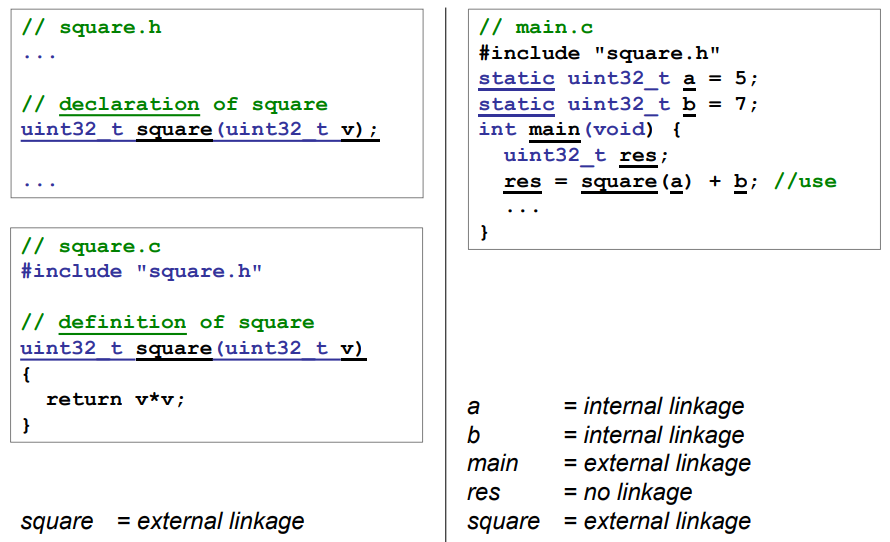
\includegraphics[width=\linewidth]{images/modular_coding_linking_lectureexample.png}
\end{example2}




\subsubsection{Linkage in C}

\begin{formula}{Linkage Types in C}
Three types of linkage:

\textbf{External Linkage}:
    \begin{itemize}
      \item Global names available to all modules
      \item Default for functions and global variables
\begin{lstlisting}[language=C, style=basesmol]
int global_var;           // External linkage
void global_func(void);   // External linkage
\end{lstlisting}
    \end{itemize}
\textbf{Internal Linkage}:
    \begin{itemize}
      \item Names only available within module
      \item Created using 'static' keyword
\begin{lstlisting}[language=C, style=basesmol]
static int module_var;    // Internal linkage
static void local_func(void); // Internal linkage
\end{lstlisting}
    \end{itemize}
\textbf{No Linkage}:
    \begin{itemize}
      \item Local variables and function parameters
      \item Scope limited to block
\begin{lstlisting}[language=C, style=basesmol]
void func(void) {
    int local_var;       // No linkage
    static int static_var; // Internal linkage
}
\end{lstlisting}
    \end{itemize}
\end{formula}



\begin{example2}{Module Interface Design}\\
Example of a well-designed modular system:

\begin{lstlisting}[language=C, style=basesmol]
// sensor.h - Public interface
typedef struct {
    uint32_t id;
    uint32_t value;
} sensor_reading_t;

void sensor_init(uint32_t id);
sensor_reading_t sensor_read(void);

// sensor.c - Implementation
static uint32_t current_sensor_id;
static uint32_t last_reading;

void sensor_init(uint32_t id) {
    current_sensor_id = id;
    last_reading = 0;
}

sensor_reading_t sensor_read(void) {
    sensor_reading_t reading;
    reading.id = current_sensor_id;
    reading.value = /* Read hardware */;
    last_reading = reading.value;
    return reading;
}
\end{lstlisting}
\end{example2}

\columnbreak




\subsubsection{Linker Input and Output}


\begin{definition}{Linker Input - Object Files}
\begin{itemize}
  \item \textbf{Code Section}: Based at address 0x0
    \begin{itemize}
      \item Program code and constant data (READONLY) of the module
    \end{itemize}
  \item \textbf{Data Section}: Based at address 0x0
    \begin{itemize}
      \item all global variables and initialized data
    \end{itemize}
  \item \textbf{Symbol Table}: References to external symbols
    \begin{itemize}
      \item All symbols with their attributes like global/local status
    \end{itemize}
  \item \textbf{Relocation Table}: Instructions for adjusting addresses:
    \begin{itemize}
      \item which bytes of the data and code sections need to be modified (and how) after merging the sections in the linking process
      \item Applied during linking process
    \end{itemize}
\end{itemize}
ARM tool chain uses ELF (Executable and Linkable Format)
\end{definition}

\begin{example2}{Object File Structure}
  File sections:
\begin{lstlisting}[language=armasm, style=basesmol]
; 1. '.text' section (Code):
0x00000000: 4604  MOV     r4,r0
0x00000002: 0040  LSLS    r0,r0,#1
0x00000004: 4420  ADD     r0,r4
; 2. '.data' section:
0x00000000: Initial values for global data
; 3. Symbol table:
; #  Name      Value   Type   Binding
  6  myFunc    0x0000  CODE   Global
  7  extVar    0x0000  DATA   Reference
; 4. Relocation entries:
Offset   Type         Symbol
0x0006   R_ARM_REL32  extVar
\end{lstlisting}
\end{example2}

\begin{concept}{Linker Operation}\\
\textbf{Linker tasks:}
\begin{itemize}
  \item Merge object file code sections
  \item Merge object file data sections
  \item Symbol Resolution: Resolve symbol references between modules
  \item Address relocation: Relocate addresses to final positions
\end{itemize}

\textbf{Linker output:} AXF = ARM executable file

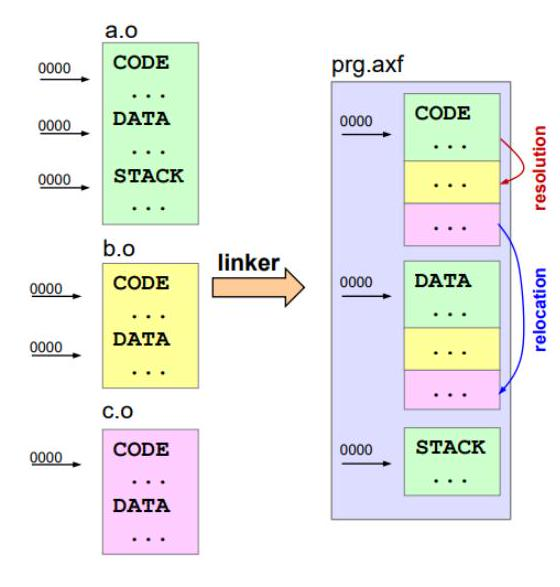
\includegraphics[width=0.8\linewidth]{images/2024_12_29_79e6b22f503fb7b4f718g-10}
\end{concept}

\begin{KR}{Symbol Resolution and Relocation}
Steps in linking process:

1. Symbol Resolution:
\begin{lstlisting}[language=armasm, style=basesmol]
    ; In module1.s
    AREA |.text|, CODE, READONLY
    EXPORT func1
func1
    ; function code
    
    ; In module2.s
    AREA |.text|, CODE, READONLY
    IMPORT func1
    BL      func1    ; Reference to resolve
\end{lstlisting}

2. Relocation:
\begin{lstlisting}[language=armasm, style=basesmol]
    ; Before relocation
    BL      func1    ; Relative offset
    
    ; After relocation
    BL      0x08000234  ; Absolute address
\end{lstlisting}
\end{KR}

\begin{example2}{Linking Multiple Modules}\\
Example of linking multiple assembly modules:

\begin{lstlisting}[language=armasm, style=basesmol]
; math_ops.s
    AREA |.text|, CODE, READONLY
    EXPORT add_values
    EXPORT multiply_values
    
add_values PROC
    ADDS R0, R0, R1
    BX LR
    ENDP
    
multiply_values PROC
    MULS R0, R1, R0
    BX LR
    ENDP
    END
    
; main.s
    AREA |.text|, CODE, READONLY
    IMPORT add_values
    IMPORT multiply_values
    EXPORT main
    
main PROC
    PUSH {R4,LR}
    MOVS R0, #5
    MOVS R1, #3
    BL add_values      ; Call add_values
    MOVS R4, R0       ; Save result
    MOVS R0, #6
    MOVS R1, #2
    BL multiply_values ; Call multiply_values
    ADD R0, R0, R4    ; Combine results
    POP {R4,PC}
    ENDP
    END
\end{lstlisting}
\end{example2}

\subsubsection{Creating and Using Libraries}



\begin{KR}{Library Creation and Use}
Steps for creating and using libraries:

1. Create library source files:
\begin{lstlisting}[language=C, style=basesmol]
// lib.h
void lib_func(int x);

// lib.c
void lib_func(int x) {
    // Implementation
}
\end{lstlisting}

2. Compile to object files:
\begin{lstlisting}[style=basesmol]
armcc -c lib.c -o lib.o
\end{lstlisting}

3. Create static library:
\begin{lstlisting}[style=basesmol]
armar --create libmy.a lib.o
\end{lstlisting}

4. Link with library:
\begin{lstlisting}[style=basesmol]
armlink main.o libmy.a -o program.axf
\end{lstlisting}
\end{KR}

\begin{example2}{Creating Static Libraries}\\
Creating and using a static library:

1. Create object files:
\begin{lstlisting}[style=basesmol]
armcc -c math_ops.c -o math_ops.o
armcc -c string_ops.c -o string_ops.o
\end{lstlisting}

2. Create static library:
\begin{lstlisting}[style=basesmol]
armar --create libutils.a math_ops.o string_ops.o
\end{lstlisting}

3. Link with library:
\begin{lstlisting}[style=basesmol]
armlink main.o libutils.a -o program.axf
\end{lstlisting}

Example C code for the library:
\begin{lstlisting}[language=C, style=basesmol]
// math_ops.h
uint32_t add_values(uint32_t a, uint32_t b);
uint32_t multiply_values(uint32_t a, uint32_t b);

// math_ops.c
uint32_t add_values(uint32_t a, uint32_t b) {
    return a + b;
}

uint32_t multiply_values(uint32_t a, uint32_t b) {
    return a * b;
}
\end{lstlisting}
\end{example2}

\begin{KR}{Creating a Multi-Module Project}\\
Steps for creating a modular program:

1. Design module structure:
\begin{itemize}
  \item Identify clear module boundaries and responsibilities 
  \item Define external interfaces between modules
  \item Plan dependencies between modules
\end{itemize}

2. Create header files (.h):
\begin{lstlisting}[language=C, style=basesmol]
// module.h
#ifndef MODULE_H_
#define MODULE_H_ 

// Public type definitions
typedef struct {
    uint32_t x;
    uint32_t y;
} point_t;

// Public function declarations
void init_module(void);
uint32_t process_point(point_t* p);

#endif
\end{lstlisting}

3. Create implementation files (.c):
\begin{lstlisting}[language=C, style=basesmol]
// module.c
#include "module.h"

// Private/static functions
static void helper_function(void) {
    // Internal implementation
}

// Public function implementations
void init_module(void) {
    // Initialize module state
}

uint32_t process_point(point_t* p) {
    helper_function();
    return p->x + p->y;
}
\end{lstlisting}

4. Create makefile/build configuration:
\begin{itemize}
  \item Define compilation and linking rules
  \item Specify dependencies between modules
  \item Configure optimization and debug settings
\end{itemize}
\end{KR}




